\documentclass[a4paper,12pt]{article}

%=========== PACKAGES ================

\usepackage[french]{babel}
\usepackage[utf8x]{inputenc}
\setlength{\headheight}{20.14264pt}
\addtolength{\topmargin}{-8.14264pt}
%\usepackage{subfigure}
%\usepackage{subcaption}
% pour gérer les positionnement d'images
\usepackage{float}
\usepackage{amsmath}
\usepackage{graphicx}
\graphicspath{{../Pictures/}}
\usepackage{wrapfig}
\usepackage[justification=centering]{caption}
%\usepackage{enumitem}
\usepackage[colorinlistoftodos]{todonotes}
\usepackage{url}

%pour les informations sur un document compilé en PDF et les liens externes / internes
\usepackage{hyperref}
\hypersetup{
    colorlinks=true,
    linkcolor=blue,
    filecolor=magenta,      
    urlcolor=cyan,
    pdftitle={Overleaf Example},
    pdfpagemode=FullScreen,
    }
%pour la mise en page des tableaux
\usepackage{amsmath}
\usepackage{array}
\usepackage{tabularx}
\usepackage[final]{pdfpages} 
\usepackage{placeins}
%pour utiliser \floatbarrier
%espacement entre les lignes
\usepackage{setspace}
%modifier la mise en page de l'abstract
%\usepackage{abstract}
%police et mise en page (marges) du document
\usepackage[T1]{fontenc}
\usepackage[top=3cm, bottom=3cm, left=3cm, right=3cm]{geometry}
%Pour les galerie d'images
\usepackage{subfig}
%\usepackage{titlesec}
\usepackage{sectsty}
\usepackage{tikz}
\usepackage{pgfplots}
\usepackage{fancyhdr}
\usepackage{stmaryrd}
\usepackage{amssymb}
\usepackage{calrsfs}
\DeclareMathOperator{\e}{e}
\parskip=3pt


%======= INFORMATION ET REGLES ==============

\hypersetup{
% Information sur le document
pdfauthor = {Gabriel Gostiaux},	% Auteurs
pdftitle = {},   % Titre du document
pdfsubject = {},		    % Sujet
pdfstartview={FitH}}% ajuste la page à la largeur de l'écran

%======= EN-TETE ET PIED DE PAGE ==========

\pagestyle{fancy}
\fancyhead[L]{TP-Hyperfréquences}
\fancyhead[R]{
\includegraphics[width=0.2\textwidth]{Logo-IOGS.png}}
\renewcommand{\headrulewidth}{1pt}
\newcommand{\HRule}{\rule{\linewidth}{0.5mm}}
\renewcommand{\footrulewidth}{1pt}
\fancyfoot[L]{Gostiaux Gabriel}
\fancyfoot[C]{}
\fancyfoot[R]{\thepage}

%======== DEBUT DU DOCUMENT ==========

\begin{document}

\begin{titlepage}
\begin{center}

% Upper part of the page. The '~' is needed because only works if a paragraph has started.

\includegraphics[width=0.75\textwidth]{Logo-IOGS.png}~\\[1.5cm]

%\textsc{\LARGE Ecole Centrale de Lyon}\\[1.5cm]

\textsc{\Large }\\[0.5cm]

% Title
\HRule \\[0.4cm]

{\bfseries
\huge \textsc{Estimation and detection using the matched filter}\\[0.5cm]
\Large Practicals 4 and 5 of Fundamental of Estimation and Detection Course}

\HRule \\[1cm]

% Author and supervisor
\begin{minipage}{0.8\textwidth}
\begin{flushleft} \large
%\emph{Groupe 4, binôme 7 :}\\[0.4 cm]
\textsc{Gostiaux} Gabriel \\[1cm]
\end{flushleft}
\end{minipage}


\textsc{\Large }\\[1cm]
"I certify that this work is original, that we have cited all the sources used, and that it contains no plagiarism."

\textsc{\Large }\\[1cm]
The following report has been edited after work made available at \url{https://github.com/GabrielGst/IO-TS}
%\includegraphics[width=0.5\textwidth]{Figures/}




\vfill

% Bottom of the page
{\large \today}

\end{center}
\end{titlepage}
\tableofcontents
\clearpage
We consider the relaxation signal of a physical process:

\[
s_{\text{clean}} = s_{0} e^{-\alpha_{0} i}, \quad i \in [0, N-1]
\]

The objective here is to estimate \(\alpha_{0}\) from a noisy signal. We consider successively two types of noises: normal (Gaussian additive) and exponential (multiplicative) noises.

\section{Estimation Under Additive Normal Noise}

We first assume that the experiment is perturbed by an additive white normal noise \( b \) and sampled at each moment \( i \in I \). Thus we know it has a standard deviation of 1 and a zero mean. We need to define an estimator of \(\alpha_{0}\), and choose the Maximum Likelihood Estimator.

\[
  s_i &= s_{clean, i} + b_i
\]

To compute the log-likelihood, we need to find an expression of the probability law of the noisy signal. Here, in the Gaussian additive noise, the resulting signal is simply a Gaussian signal centered on the true signal and with the variance of the noise.

\[
P_{\alpha_0}(s_i) = \frac{1}{\sqrt{2\pi} \sigma} \times \exp\left(-\frac{(s_i - s_0 \times \exp(-\alpha_0 i))^2}{2\sigma^2}\right)
\]

\begin{figure}[h]
  \centering
  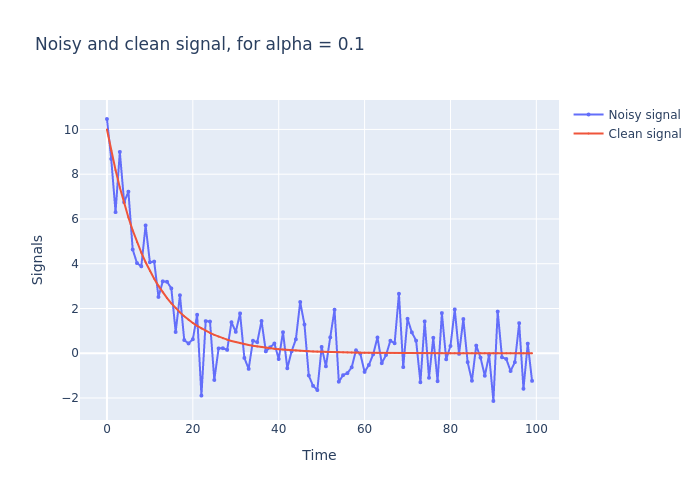
\includegraphics[scale=0.4]{../Pictures/IO24 - TS - lab 2.2 - estimation_8_0.png}
  \caption{Noisy and clean signal}
\end{figure}

\pagebreak

One can then obtain the log-likelihood \( l_\alpha \)

\[
l_{\alpha} = \sum_{i \in I} ln(P_{\alpha_0}(s_i)) = -\frac{N}{2} \times \log(2\pi\sigma^2) - \frac{1}{2\sigma^2} \sum_{i=0}^{N-1} \left[s_i - s_0 \times \exp(-\alpha i)\right]^2
\]

\begin{figure}[h]
  \centering
  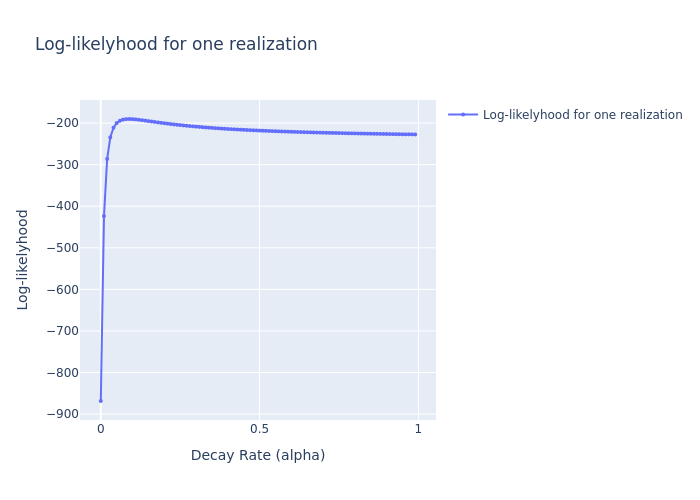
\includegraphics[scale=0.4]{../Pictures/IO24 - TS - lab 2.2 - estimation_8_1.png}
  \caption{log-likelihood}
\end{figure}
  
\begin{figure}
  \centering
  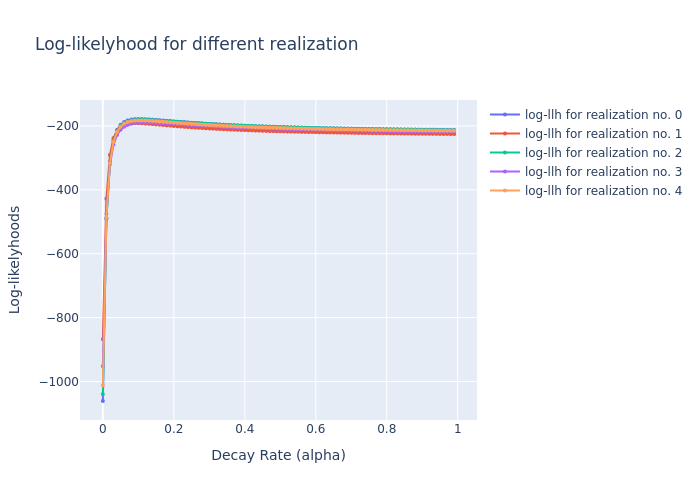
\includegraphics[scale=0.4]{../Pictures/IO24 - TS - lab 2.2 - estimation_8_2.png}
  \caption{log-likelihood for multiple realizations}
\end{figure}

In regard of the chart, one can assume this function of \(\alpha\) admits a maximum. On the
figure, we can estimate \(\alpha_0 = 0.1\). Thus one could define the MLE, which is then obtained for \(\frac{\partial l_{\alpha}}{\partial \alpha} = 0\) and should attain the Cramer Rao Lower Bound (CRLB) defined with \(\frac{\partial^2 l_{\alpha}}{\partial \alpha^2}\) because the PDF is part of the exponential family, thus the ML estimator is not efficient.

\[
\frac{\partial l_{\alpha}}{\partial \alpha} = \frac{s_0}{\sigma^2} \sum_{i=0}^{N-1} \left[i \times \exp(-\alpha_0 i) \times \left(s_i - s_0 \times \exp(-\alpha_0 i)\right)\right] = 0
\]

As can be seen in the formula, one can only computes numerically the estimator.

Let's find the expression of the Cramer-Rao Lower Bound (CRLB) for the estimation of \(\alpha_{0}\) by computing the second derivative.

\[
\frac{\partial^2 l_{\alpha}}{\partial^2 \alpha} = - \frac{s_0}{\sigma^2} \sum_{i=0}^{N-1} \left[i^2 \times \exp(-\alpha_0 i) \times \left(s_i - 2 \times s_0 \times \exp(-\alpha_0 i)\right)\right]
\]

We note that the square root of the Signal to Noise Ratio \(\frac{s_{0}}{\sigma}\) appears in the expression, however it does not look like it could be computed analyticaly. Assuming the mean of the measured signal is the clean signal, the expression of the CRLB can be simplified using:

\[
\sum_{n=0}^{+\infty} n^{2} q^{n} = \frac{q(1+q)}{(1-q)^{3}}, \quad q < 1
\]

And we have:

\[
\frac{\partial^2 l_{\alpha}}{\partial^2 \alpha} = -\frac{s_0^2}{\sigma^2} \sum_{i=0}^{+\infty} \left[i^2 \times \exp(-2\alpha_0 i)\right]
\]

The CRLB is then equal to:

\[
\text{CRLB} = -\mathbb{E}\left(1 / \frac{\partial^2 l_{\alpha}}{\partial^2 \alpha}\right) = \frac{\sigma^2}{s_0^2} \times \frac{(1-e^{-2\alpha_0})^3}{e^{-2\alpha_0}(1+e^{-2\alpha_0})}
\]

\begin{center}\rule{0.5\linewidth}{0.5pt}\end{center}

Numerically, we compute the \textbf{Decay estimator that minimizes the function} to be equal to \textbf{0.10242188}. This value is almost identical to the input parameter ( \( 0.1 \) ). We then estimate the statistical mean and variance of the estimator with a Monte Carlo simulation.

\begin{figure}[h]
  \centering
  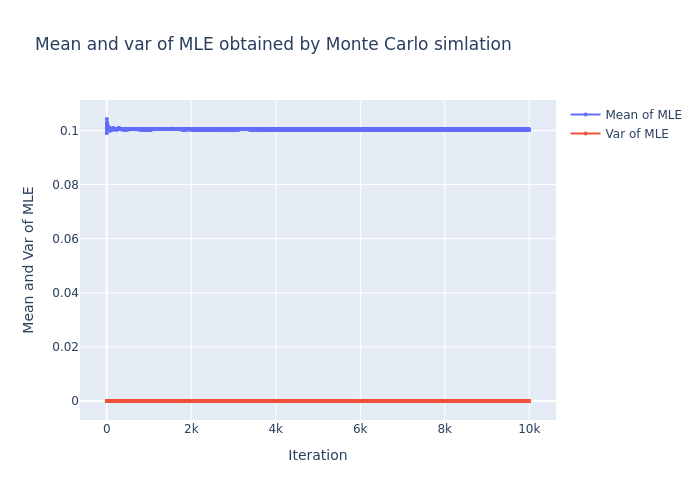
\includegraphics[scale=0.4]{../Pictures/IO24 - TS - lab 2.2 - estimation_14_0.png}
  \caption{Monte Carlo simulation}
\end{figure}

From the simulation one knows the CRLB for a decay rate equal to \( 0.1 \) is \( 4.000028574288418 \times 10^{-5} \). Since the variance computed analyticaly equals the CRLB, the estimator is efficient, and itis not biased since it does not differ from the exact theoretical valueas shown by the Monte Carlo simulation. The efficiency of the estimator could be predicted due to its belonging to the exponential family and that it was unbiased.

\pagebreak

\section{Exponential Case}

We now consider that the signal (2.1) is perturbed by exponential noise. One can remember that for such a process (with mean \(I\)) the probability density is:

\[
P(x) = \frac{1}{I} \exp \left[-\frac{x}{I}\right]
\]

The resulting random variable follows an exponential probability law shifted by the deterministic signal:

\[
P_{\alpha}(s_i) = \frac{1}{s_{\text{clean}}} \exp \left(-\frac{s_i}{s_{\text{clean}}}\right)
\]

\begin{figure}[h]
  \centering
  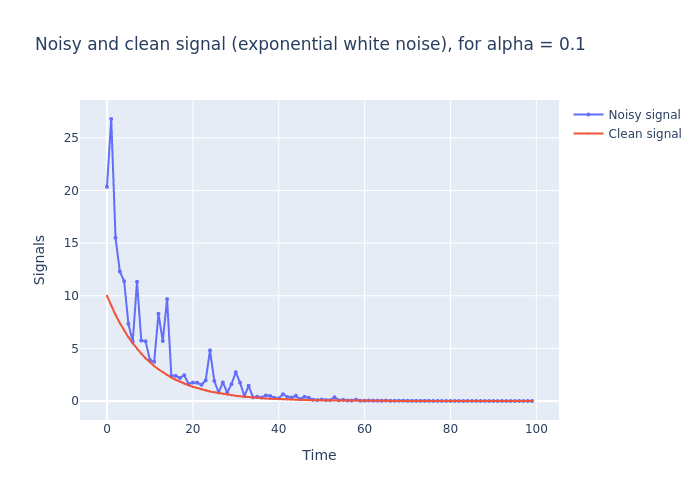
\includegraphics[scale=0.4]{../Pictures/IO24 - TS - lab 2.2 - estimation_21_0.png}
  \caption{Noisy and clean exponential signal}
\end{figure}

\pagebreak

Then one can compute the log-likelihood and compute the derivative along \( \alpha \) :

\[
\begin{aligned}
l_{\alpha} &= -\sum_{i \in I} \ln \left(s_{\text{clean}}\right) - \sum_{i \in I} \left(\frac{s_i}{s_{\text{clean}}}\right) \\
\frac{\partial l_{\alpha}}{\partial \alpha} &= \frac{\partial}{\partial \alpha}\left[-\sum_{i \in I} \ln \left(s_0 e^{-\alpha i}\right) - \sum_{i \in I} \frac{s_i}{s_0} e^{\alpha i}\right] \\
\frac{\partial l_{\alpha}}{\partial \alpha} &= \frac{\partial}{\partial \alpha}\left[-N \ln (s_0) + \alpha \sum_{i \in I} i - \sum_{i \in I} \frac{s_i}{s_0} e^{\alpha i}\right]
\end{aligned}
\]

\begin{figure}[h]
  \centering
  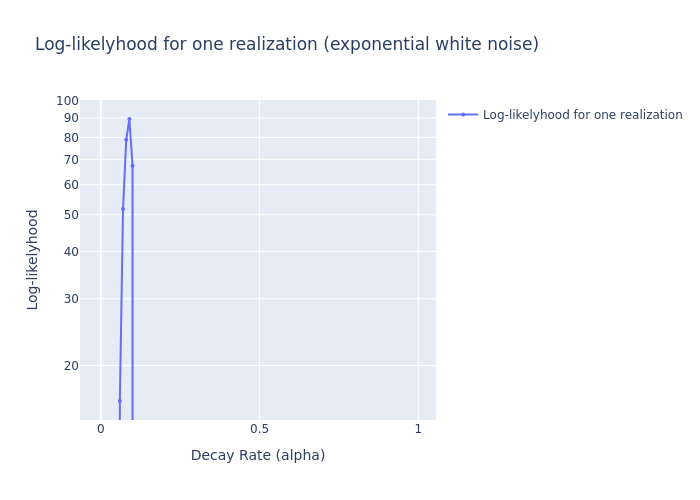
\includegraphics[scale=0.4]{../Pictures/IO24 - TS - lab 2.2 - estimation_21_1.png}
  \caption{log-likelihood}
\end{figure}
  
\begin{figure}
  \centering
  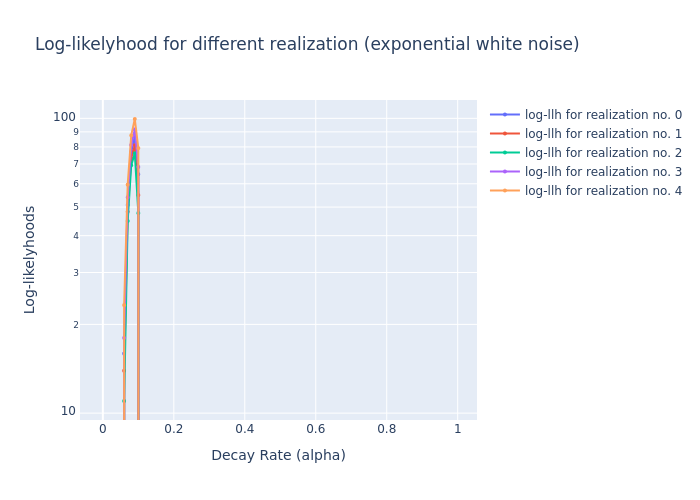
\includegraphics[scale=0.4]{../Pictures/IO24 - TS - lab 2.2 - estimation_21_2.png}
  \caption{log-likelihood, multiple realization}
\end{figure}

Again one knows the MLE can be obtained. The derivative results in:

\[
\begin{aligned}
\frac{\partial l_{\alpha}}{\partial \alpha} & = \sum_{i \in I} i - \sum_{i \in I} \frac{s_i}{s_0} i e^{\alpha i} \\
0 &= \sum_{i \in I} i - \sum_{i \in I} \frac{s_i}{s_0} i e^{\alpha_{0} i} \\
0 &= \sum_{i \in I} i \left( 1 - \frac{s_i}{s_0} e^{\alpha_{0} i}\right)
\end{aligned}
\]

Once again, the results needs to be computed numerically. A second derivation gives access to the CRLB :

\[
\begin{aligned}
\frac{\partial^2 l_{\alpha}}{\partial^2 \alpha} & = -\frac{1}{s_0} \sum s_i i^2 e^{\alpha i} \\
\left\langle \frac{\partial^2 l_{\alpha}}{\partial^2 \alpha}\right\rangle & = -\frac{1}{s_0} \sum \left\langle s_i \right\rangle i^2 e^{\alpha i} \\
& = -\sum i^2
\end{aligned}
\]

And since:

\[
\sum_{n=0}^{N} n^{2} = \frac{N(N+1)(2N+1)}{6}
\]

\[
\text{CRLB} = -\frac{1}{\left\langle \frac{\partial^2 L_{\alpha}}{\partial^2 \alpha}\right\rangle} = \frac{6}{N(N+1)(2N+1)}
\]

This time, the CRLB depends only on the size of the sample, so that the minimum variance of the estimator can be theoritically lowered by using a larger sample.

\begin{center}\rule{0.5\linewidth}{0.5pt}\end{center}

Numerically, we compute the \textbf{Decay estimator that minimizes the function} to be equal to \textbf{0.08886719}. This value is almost identical to the input parameter ( \(0.9 \) ). We then estimate the statistical mean and variance of the estimator with a Monte Carlo simulation.

\begin{figure}[h]
\centering
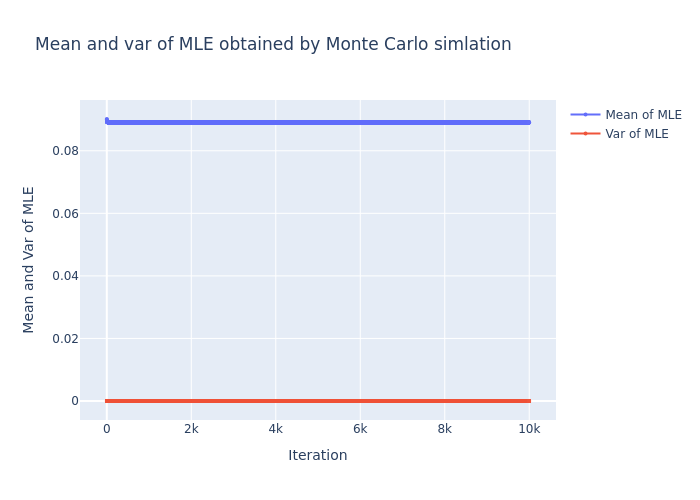
\includegraphics[scale=0.4]{../Pictures/IO24 - TS - lab 2.2 - estimation_27_0.png}
\caption{Monte Carlo simulation}
\end{figure}

Since the variance equals the CRLB, the estimator is efficient, and itis not biased since it does not differ from the exact theoretical value as shown by the Monte Carlo simulation. Again this could be predicted due to the belonging to the exponential family and the unbiased nature of the estimator.


\section{Estimator Comparison}
What changes if we decide to use one estimator for the other signal ? Let's try to use the estimator for the signal perturbed by a gaussian noise to estimate the \( \alpha \) parameter of the signal perturbed by the exponential noise.

With the previous method (Monte Carlo Simulation), one can show that the estimator is now biased and that its variance will not reach the Cramer Rao Lower Bound.

\section{Conclusion}

This analysis showed that in the case of a clean signal representing an exponential decay, perturbed first by a gaussian exponential white noise, and then by an exponential white noise, the estimators defined by the Maximum of Likelihood are unbiased and efficients.

This practical highlighted the role of estimators to analyse time series signals. Indeed, it is of importance in physics for engineering purposes, but it can also be applied to other types of time series, for example financial data.
\listoffigures
\end{document}
